\documentclass[10pt,leqno]{article}

\usepackage[%
  tmargin=1.2in,bmargin=1.2in,%
  lmargin=1.8in,rmargin=1.8in,%
]{geometry}
\usepackage{fancyhdr}
\usepackage{titlesec}
\usepackage{appendix}
\usepackage{microtype}
\usepackage[hyphens]{url}
\usepackage{enumitem}
\usepackage{xspace}
\usepackage{etoolbox}
\usepackage{ifthen}
\usepackage{tikz}
\usepackage{tikz-cd}

\usepackage{amsmath}
\definecolor{darkred}{rgb}{0.5,0.0,0.0}
\usepackage[%
  colorlinks,%
  linkcolor=darkred,%
  citecolor=darkred,%
  urlcolor=darkred,%
]{hyperref}
\usepackage{amsthm,amssymb}
% \usepackage[lining,semibold]{libertine}
% \usepackage{textcomp,stmaryrd}
% \usepackage[libertine,cmintegrals,bigdelims]{newtxmath}
% \useosf
% \usepackage[%
%   cal=boondox, calscaled=0.97,%
%   bb=boondox, bbscaled=0.98,%
% ]{mathalfa}
\usepackage{cleveref}

\frenchspacing
\urlstyle{rm}

\AtBeginDocument{%
  \setlength{\abovedisplayskip}{1.5ex plus 0.3ex minus 0.3ex}%
  \setlength{\abovedisplayshortskip}{1.0ex plus 0.3ex minus 0.3ex}%
  \setlength{\belowdisplayskip}{1.5ex plus 0.3ex minus 0.3ex}%
  \setlength{\belowdisplayshortskip}{1.0ex plus 0.3ex minus 0.3ex}%
}

\let\theoldbibliography\thebibliography
\renewcommand{\thebibliography}[1]{%
  \theoldbibliography{#1}%
  \setlength{\parskip}{0ex}
  \setlength{\itemsep}{0.5ex plus 0.2ex minus 0.2ex}
  \small
}

\pagestyle{fancy}
\renewcommand{\headrulewidth}{0pt}
\renewcommand{\footrulewidth}{0pt}
\fancyhf{}
\fancyfoot[C]{\small\thepage}

\renewcommand{\title}[1]{\newcommand{\thetitle}{#1}}
\renewcommand{\author}[1]{\newcommand{\theauthor}{#1}}
\renewcommand{\date}[1]{\newcommand{\thedate}{#1}}

\renewcommand{\maketitle}{%
  \begin{center}
    {\bfseries\MakeUppercase{%
      \thetitle}}\\[2.5ex]
    {\footnotesize\MakeUppercase{%
      \theauthor}}\\[2.5ex]
    \ifthenelse{\equal{\thedate}{}}{}{%
      \small%
      \setlength{\tabcolsep}{0.2em}%
      \begin{tabular}{rl}
        original: & \thedate \\
        updated: & \today
      \end{tabular}
    }
  \end{center}
  \vspace{2.5ex}
  \thispagestyle{fancy}
}

%%%%%%%%%%%%%%%%%%%%%%%%%%%%%%%%%%%%%%%%%%%%%%%%%%%%%%%%%%%%%%%%%%%%%%

\cspreto{section}{\setcounter{equation}{0}}

\titleformat{\section}{\centering\scshape}{\thesection.}{0.4em}{}
\titlespacing{\section}{0pt}{*4}{*1}
\titleformat{\subsection}{\scshape}{\thesubsection.}{0.4em}{}
\titlespacing{\subsection}{0pt}{*2.5}{*1}

% Display format for equations
\newcommand{\crefeqfmt}[1]{
  \crefformat{#1}{(##2##1##3)}
  \Crefformat{#1}{(##2##1##3)}
  \crefrangeformat{#1}{(##3##1##4--##5##2##6)}
  \Crefrangeformat{#1}{(##3##1##4--##5##2##6)}
  \crefmultiformat{#1}{(##2##1##3}{, ##2##1##3)}{, ##2##1##3}{, ##2##1##3)}
  \Crefmultiformat{#1}{(##2##1##3}{, ##2##1##3)}{, ##2##1##3}{, ##2##1##3)}
  \crefrangemultiformat{#1}{(##3##1##4--##5##2##6}{, ##3##1##4--##5##2##6)}{, ##3##1##4--##5##2##6}{, ##3##1##4--##5##2##6)}
  \Crefrangemultiformat{#1}{(##3##1##4--##5##2##6}{, ##3##1##4--##5##2##6)}{, ##3##1##4--##5##2##6}{, ##3##1##4--##5##2##6)}
}
% Display format for sections
\newcommand{\crefsecfmt}[1]{%
  \crefformat{#1}{\S##2##1##3}
  \Crefformat{#1}{\S##2##1##3}
  \crefrangeformat{#1}{\S\S##3##1##4--##5##2##6}
  \Crefrangeformat{#1}{\S\S##3##1##4--##5##2##6}
  \crefmultiformat{#1}{\S\S##2##1##3}{ and~##2##1##3}{, ##2##1##3}{ and~##2##1##3}
  \Crefmultiformat{#1}{\S\S##2##1##3}{ and~##2##1##3}{, ##2##1##3}{ and~##2##1##3}
  \crefrangemultiformat{#1}{\S\S##3##1##4--##5##2##6}{ and~##3##1##4--##5##2##6}{, ##3##1##4--##5##2##6}{ and~##3##1##4--##5##2##6}
  \Crefrangemultiformat{#1}{\S\S##3##1##4--##5##2##6}{ and~##3##1##4--##5##2##6}{, ##3##1##4--##5##2##6}{ and~##3##1##4--##5##2##6}
}
\crefeqfmt{equation}
\crefeqfmt{enumi}
\crefeqfmt{enumii}
\crefsecfmt{section}
\crefsecfmt{subsection}
\crefsecfmt{appendix}
\crefname{part}{Part}{Parts}
\crefname{chapter}{Chapter}{Chapters}
\crefname{figure}{Figure}{Figures}

\makeatletter

\newcommand{\thmnumfont}{\bfseries}
\newcommand{\thmheadfont}{\bfseries}
\newcommand{\thmnotefont}{\bfseries}
\newcommand{\thmhorizspace}{0.4em}

\def\swappedhead#1#2#3{%
  \thmnumber{\@upn{{\thmnumfont#2}}\@ifnotempty{#1}{.\hspace{0.25em}}}%
  \thmheadfont\thmname{#1}%
  \@ifnotempty{#3}{\ \thmnote{\thmnotefont(#3)}}%
}
\swapnumbers

\newtheoremstyle{block}%
  {2.0ex plus 0.2ex minus 0.1ex}% Space above
  {2.0ex plus 0.2ex minus 0.1ex}% Space below
  {} % Body font
  {} % Indent amount
  {\thmheadfont} % Theorem head font
  {.} % Punctuation after theorem head
  {\thmhorizspace} % Space after theorem head
  {} % Theorem head spec (can be left empty, meaning ‘normal’)

\renewenvironment{proof}[1][Proof]{\par
  \pushQED{\qed}%
  \normalfont%
  \topsep1ex plus 0.2ex minus 0.1ex\relax%
  \labelsep \thmhorizspace\relax%
  \trivlist
  \item[\hskip\labelsep\thmheadfont
    #1\@addpunct{.}]\ignorespaces
}{%
  \popQED\endtrivlist\@endpefalse%
}

\makeatother

\theoremstyle{block}

\newcommand{\defthm}[2]{%
  \newtheorem{#1}[equation]{#2}%
  \crefeqfmt{#1}%
  \newtheorem*{#1*}{#2}%
}

\defthm{algorithm}{Algorithm}
\defthm{conjecture}{Conjecture}
\defthm{construction}{Construction}
\defthm{convention}{Convention}
\defthm{corollary}{Corollary}
\defthm{definition}{Definition}
\defthm{definitions}{Definitions}
\defthm{example}{Example}
\defthm{examples}{Examples}
\defthm{exercise}{Exercise}
\defthm{fact}{Fact}
\defthm{intuition}{Intuition}
\defthm{lemma}{Lemma}
\defthm{notation}{Notation}
\defthm{nothing}{}
\defthm{proposition}{Proposition}
\defthm{question}{Question}
\defthm{remark}{Remark}
\defthm{remarks}{Remarks}
\defthm{situtation}{Situation}
\defthm{theorem}{Theorem}

\setlist{%
  leftmargin=2.5em, parsep=0ex, listparindent=\parindent,
  itemsep=1.0ex, topsep=1.0ex,%
}

\setlist[enumerate, 1]{%
  label=(\alph*),%
  ref=\alph*,%
  widest=d,%
}
\setlist[enumerate, 2]{%
  label=(\roman*),%
  ref=\theenumi.\roman*,%
}
\setlist[itemize, 1]{%
  label=$\vcenter{\hbox{\footnotesize$\bullet$}}$,%
}
\setlist[itemize, 2]{label=--}

%%%%%%%%%%%%%%%%%%%%%%%%%%%%%%%%%%%%%%%%%%%%%%%%%%%%%%%%%%%%%%%%%%%%%%

\makeatletter

\let\ea\expandafter

\newcount\foreachcount

\def\foreachletter#1#2#3{\foreachcount=#1
  \ea\loop\ea\ea\ea#3\@alph\foreachcount
  \advance\foreachcount by 1
  \ifnum\foreachcount<#2\repeat}

\def\foreachLetter#1#2#3{\foreachcount=#1
  \ea\loop\ea\ea\ea#3\@Alph\foreachcount
  \advance\foreachcount by 1
  \ifnum\foreachcount<#2\repeat}

% Roman: \rA is \mathrm{A}
\def\definerm#1{%
  \ea\gdef\csname r#1\endcsname{\ensuremath{\mathrm{#1}}\xspace}}
\foreachLetter{1}{27}{\definerm}
\foreachletter{1}{27}{\definerm}
% Script: \sA is \mathscr{A}
\def\definescr#1{%
  \ea\gdef\csname s#1\endcsname{\ensuremath{\mathscr{#1}}\xspace}}
\foreachLetter{1}{27}{\definescr}
% Calligraphic: \cA is \mathcal{A}
\def\definecal#1{%
  \ea\gdef\csname c#1\endcsname{\ensuremath{\mathcal{#1}}\xspace}}
\foreachLetter{1}{27}{\definecal}
% Bold: \bA is \mathbf{A}
\def\definebold#1{%
  \ea\gdef\csname b#1\endcsname{\ensuremath{\mathbf{#1}}\xspace}}
\foreachLetter{1}{27}{\definebold}
% Blackboard Bold: \lA is \mathbb{A}
\def\definebb#1{%
  \ea\gdef\csname l#1\endcsname{\ensuremath{\mathbb{#1}}\xspace}}
\foreachLetter{1}{27}{\definebb}
% Fraktur: \ka is \mathfrak{a}, \kA is \mathfrak{A}
\def\definefrak#1{%
  \ea\gdef\csname k#1\endcsname{\ensuremath{\mathfrak{#1}}\xspace}}
\foreachletter{1}{27}{\definefrak}
\foreachLetter{1}{27}{\definefrak}
% Sans serif: \iA \is \mathsf{A}
\def\definesf#1{%
  \ea\gdef\csname i#1\endcsname{\ensuremath{\mathsf{#1}}\xspace}}
\foreachletter{1}{6}{\definesf}
\foreachletter{7}{14}{\definesf}
\foreachletter{15}{27}{\definesf}
\foreachLetter{1}{27}{\definesf}
% Bar: \Abar is \overline{A}, \abar is \overline{a}
\def\definebar#1{%
  \ea\gdef\csname #1bar\endcsname{\ensuremath{\overline{#1}}\xspace}}
\foreachLetter{1}{27}{\definebar}
\foreachletter{1}{8}{\definebar} % \hbar is something else!
\foreachletter{9}{15}{\definebar} % \obar is something else!
\foreachletter{16}{27}{\definebar}
% Tilde: \Atil is \widetilde{A}, \atil is \widetilde{a}
\def\definetil#1{%
  \ea\gdef\csname #1til\endcsname{\ensuremath{\widetilde{#1}}\xspace}}
\foreachLetter{1}{27}{\definetil}
\foreachletter{1}{27}{\definetil}
% Hats: \Ahat is \widehat{A}, \ahat is \widehat{a}
\def\definehat#1{%
  \ea\gdef\csname #1hat\endcsname{\ensuremath{\widehat{#1}}\xspace}}
\foreachLetter{1}{27}{\definehat}
\foreachletter{1}{27}{\definehat}
% Checks: \Achk is \widecheck{A}, \achk is \widecheck{a}
\def\definechk#1{%
  \ea\gdef\csname #1chk\endcsname{\ensuremath{\widecheck{#1}}\xspace}}
\foreachLetter{1}{27}{\definechk}
\foreachletter{1}{27}{\definechk}
% Underline: \Aund is \underline{A}, \aund is \underline{a}
\def\defineul#1{%
  \ea\gdef\csname #1und\endcsname{\ensuremath{\underline{#1}}\xspace}}
\foreachLetter{1}{27}{\defineul}
\foreachletter{1}{27}{\defineul}

\makeatother

%%%%%%%%%%%%%%%%%%%%%%%%%%%%%%%%%%%%%%%%%%%%%%%%%%%%%%%%%%%%%%%%%%%%%%

\usetikzlibrary{calc,decorations.pathmorphing,shapes,arrows}
\tikzcdset{
  arrow style=tikz,
  diagrams={>={stealth}},
}

\newcommand{\arrlen}{1em}
\renewcommand{\to}{\mathrel{\tikz[baseline]%
    \draw[>=stealth,->](0,0.5ex)--(\arrlen,0.5ex);}}
\newcommand{\from}{\mathrel{\tikz[baseline]%
    \draw[>=stealth,<-](0,0.5ex)--(\arrlen,0.5ex);}}
\renewcommand{\mapsto}{\mathrel{\tikz[baseline]%
    \draw[>=stealth,|->](0,0.5ex)--(\arrlen,0.5ex);}}
\newcommand{\inj}{\mathrel{\tikz[baseline]%
    \draw[>=stealth,right hook->](0,0.5ex)--(\arrlen,0.5ex);}}
\newcommand{\surj}{\mathrel{\tikz[baseline]%
    \draw[>=stealth,->>](0,0.5ex)--(\arrlen,0.5ex);}}
\newcommand{\fromto}{\mathrel{%
  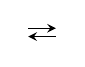
\begin{tikzpicture}[baseline]%
    \draw[>=stealth,<-](0,0.15ex)--(\arrlen,0.15ex);%
    \draw[>=stealth,->](0,0.85ex)--(\arrlen,0.85ex);%
  \end{tikzpicture}}}
\newcommand{\doubto}{\mathrel{%
  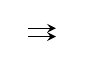
\begin{tikzpicture}[baseline]%
    \draw[>=stealth,->](0,0.15ex)--(\arrlen,0.15ex);%
    \draw[>=stealth,->](0,0.85ex)--(\arrlen,0.85ex);%
  \end{tikzpicture}}}
\newcommand{\lblto}[1]{\mathrel{%
    \begin{tikzpicture}[baseline= {( $ (current bounding box.south) + (0,-0.5ex) $ )}]
      \node[inner sep=.4ex] (a) {\,$\scriptstyle #1$\,};
      \draw[>=stealth,->] (a.south west) -- (a.south east);
    \end{tikzpicture}}}
\newcommand{\isoto}{\lblto{\sim}}

\newcommand{\simpl}[3]{
  \begin{tikzcd}[ampersand replacement=\&, column sep=small]
    #1 \&
    #2 \ar[l, shift right=0.35ex]
       \ar[l, shift left=0.35ex] \&
    #3 \ar[l, shift right=0.70ex]
       \ar[l, shift left=0.70ex]
       \ar[l] \&
    \cdots \ar[l, shift right=0.35ex]
           \ar[l, shift left=0.35ex]
           \ar[l, shift right=1.05ex]
           \ar[l, shift left=1.05ex]
  \end{tikzcd}
}
\newcommand{\cosimpl}[3]{
  \begin{tikzcd}[ampersand replacement=\&, column sep=small]
    #1 \ar[r, shift right=0.35ex]
       \ar[r, shift left=0.35ex] \&
    #2 \ar[r, shift right=0.70ex]
       \ar[r, shift left=0.70ex]
       \ar[r] \&
    #3 \ar[r, shift right=0.35ex]
       \ar[r, shift left=0.35ex]
       \ar[r, shift right=1.05ex]
       \ar[r, shift left=1.05ex] \&
    \cdots
  \end{tikzcd}
}

\newcommand{\tto}{\mathrel{\tikz[baseline]%
    \draw[>=stealth,->,double, double distance = 0.3ex](0,0.5ex)--(\arrlen,0.5ex);}}
\newcommand{\doubfrom}{\mathrel{%
  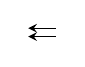
\begin{tikzpicture}[baseline]%
    \draw[>=stealth,<-](0,0.15ex)--(\arrlen,0.15ex);%
    \draw[>=stealth,<-](0,0.85ex)--(\arrlen,0.85ex);%
  \end{tikzpicture}}}
\newcommand{\tripfrom}{\mathrel{%
  
\begin{tikzpicture}[baseline]%
    \draw[>=stealth,<-](0,0.00ex)--(\arrlen,0.00ex);%
    \draw[>=stealth,<-](0,0.50ex)--(\arrlen,0.50ex);%
    \draw[>=stealth,<-](0,1.00ex)--(\arrlen,1.00ex);%
  \end{tikzpicture}}}


\renewcommand{\l}{\left}
\renewcommand{\r}{\right}
\newcommand{\f}{\frac}
\renewcommand{\o}{\overline}
\renewcommand{\u}{\underline}
\newcommand{\til}{\widetilde}
\renewcommand{\hat}{\widehat}
\newcommand{\del}{\partial}
\newcommand{\dash}{\text{-}}
\renewcommand{\c}{\colon}
\newcommand{\lc}{\,:\!}
\newcommand{\ce}{\coloneq}%{\mathrel{:=}}
\newcommand{\ec}{\eqcolon}%{\mathrel{=:}}
\newcommand{\iso}{\simeq}
\newcommand{\dual}{\vee}
\newcommand{\ldb}{\llbracket}
\newcommand{\rdb}{\rrbracket}

\newcommand{\Obj}{\operatorname{Obj}}
\newcommand{\Hom}{\operatorname{Hom}}
\newcommand{\Map}{\operatorname{Map}}
\newcommand{\Fun}{\operatorname{Fun}}
\newcommand{\Aut}{\operatorname{Aut}}
\newcommand{\Iso}{\operatorname{Iso}}
\renewcommand{\id}{\mathrm{id}}
\renewcommand{\im}{\operatorname{im}}
\newcommand{\op}{\mathrm{op}}
\newcommand{\univ}{\mathrm{univ}}
\newcommand{\colim}{\operatorname*{colim}}
\newcommand{\dlim}{\displaystyle\lim}
\newcommand{\dcolim}{\displaystyle\colim}
\newcommand{\Spec}{\operatorname{Spec}}
\newcommand{\Spf}{\operatorname{Spf}}

%%%%%%%%%%%%%%%%%%%%%%%%%%%%%%%%%%%%%%%%%%%%%%%%%%%%%%%%%%%%%%%%%%%%%%


\title{Math 216A Homework 7}
\author{Arpon Raksit}
\date{November 10, 2016}

\numberwithin{block}{section}

%%%%%%%%%%%%%%%%%%%%%%%%%%%%%%%%%%%%%%%%%%%%%%%%%%%%%%%%%%%%%%%%%%%%%%

\begin{document}
\maketitle

\newcommand{\Psh}{\operatorname{Psh}}
\newcommand{\Shv}{\operatorname{Shv}}

%%%%%%%%%%%%%%%%%%%%%%%%%%%%%%%%%%%%%%%%%%%%%%%%%%%%%%%%%%%%%%%%%%%%%%

\section{Group actions on schemes}

\subsection*{Part (i)}

Let $G$ be a (discrete) group.

\begin{nothing}
  \label{action-as-functor}
  Let $\rB G$ denote the category with one object whose automorphism group is $G$ (and with no other objects or morphisms). Let $\sC$ be a category, and suppose given a left-action of $G$ on an object $C \in \sC$, i.e. a group homomorphism $G \to \Aut(C)$. (All of the following goes through for right-actions as well, by replacing $G$ with $G^\op$.) Observe that this data is equivalent to a functor $\alpha \c \rB G \to \sC$ taking the unique object of $\rB G$ to $C$. We let $\alpha_g \c C \to C$ denote the action of $g \in G$ on $C$.

  \begin{subdefinition}
    \label{invariants-as-limit}
    In this generality, the \emph{object of invariants} of this action, denoted $C^G$, is defined to be the limit of this functor $\alpha$ (if it exists), and the \emph{quotient object} of this action, denoted $C_G$, is defined to be the colimit of this functor $\alpha$ (if it exists).

    Unwrapping the definitions of limit and colimit, $C^G$ is the universal object of $\sC$ equipped with a map $\iota \c C^G \to C$ satisfying $\alpha_g\iota = \iota$ for all $g \in G$, and $C_G$ is the universal object of $\sC$ equipped with a map $\pi \c C \to C_G$ satisfying $\pi\alpha_g = \pi$ for all $g \in G$.
  \end{subdefinition}
\end{nothing}

\begin{nothing}
  \label{ringed-space-quotient}
  Let $(Z,\sO_Z)$ be a ringed space with a right-action of $G$ (in the category of ringed spaces). That is, we have for each $g \in G$ an automorphism $\alpha_g \c Z \isoto Z$ and an isomorphism $\phi_g \c \sO_Z \isoto (\alpha_g)_*\sO_Z$, and for pairs $g,h \in G$ we have $\alpha_{gh} = \alpha_h\alpha_g$ and a commutative diagram
  \begin{equation}
    \label{sheaf-action}
    \begin{tikzcd}
      \sO_Z \ar[r, "\phi_h"] \ar[d, "\phi_{gh}", swap] &
      (\alpha_h)_*\sO_Z \ar[d, "(\alpha_h)_*(\phi_g)"] \\
      (\alpha_{gh})_*\sO_Z \ar[r, "\sim"] &
      (\alpha_h)_*(\alpha_g)_*\sO_Z.
    \end{tikzcd}
  \end{equation}
  
  \begin{subconstruction}
    \label{ringed-space-quotient-constr}  
    Now let $Z/G$ be a the quotient space, $\pi \c Z \to Z/G$ the quotient map.  By definition we have that $\pi \alpha_g = \pi$ for each $g \in G$, and hence pushing forward the maps $\phi_g$ in $\pi$ gives us automorphisms
    \[
      \psi_g \ce \pi_*(\phi_g) \c \pi_*(\sO_Z) \isoto \pi_*(\alpha_g)_*\sO_Z \iso \pi_*\sO_Z;
    \]
    and \cref{sheaf-action} implies that $\psi_{gh} = \psi_g\psi_h$ for $g,h \in G$, so these automorphisms determine a left-action of $G$ on $\pi_*(\sO_Z)$ in the category of sheaves of rings on $Z/G$. 

    Define $\sO_{Z/G} \ce (\pi_*\sO_Z)^G$ to be the invariants of this action (in the category of sheaves of rings on $Z/G$ (which admits all limits), as defined in \cref{invariants-as-limit}). There is by definition a canonical map $\iota \c \sO_{Z/G} \to \pi_*\sO_Z$ . Together with the quotient map this gives us a map of ringed spaces $(\pi,\iota) \c (Z,\sO_Z) \to (Z/G,\sO_{Z/G})$.
  \end{subconstruction}

  \begin{sublemma}
    \label{invariants-identification}
    The map $\iota \c \sO_{Z/G} \to \pi_*\sO_Z$ can be identified with the inclusion of the presheaf of $G$-invariant sections of $\pi_*\sO_Z$.

    \begin{proof}
      This follows from the facts that the forgetful functors from
      \begin{itemize}
      \item the category of sheaves of sets on a space to the category of presheaves of sets on that space,
      \item and the category of rings to the category of sets
      \end{itemize}
      both preserve limits.
    \end{proof}
  \end{sublemma}

  \begin{subproposition}
    \label{ringed-space-quotient-univ}
    The map $(\pi,\iota) \c (Z,\sO_Z) \to (Z/G,\sO_{Z/G})$ exhibits $(Z/G,\sO_{Z/G})$ as the quotient object $(Z,\sO_Z)_G$ in the category of ringed spaces.

    \begin{proof}
      Let $(Z',\sO_{Z'})$ be any ringed space. A map of ringed spaces $(Z/G,\sO_{Z/G}) \to (Z',\sO_{Z'})$ is given by a map of spaces $\rho \c Z/G \to Z'$ and a map of sheaves of rings $\theta \c \sO_{Z'} \to \rho_*\sO_{Z/G}$.
      
      The quotient space $Z/G$ is a quotient object in the category of topological spaces, so giving $\rho$ is equivalent to giving the map $\til\rho \ce \rho\pi \c Z \to Z'$ satisfying $\til\rho\alpha_g = \til\rho$ for $g \in G$.

      Since $\rho_*$ preserves limits (it is a right adjoint) and $\sO_{Z/G}$ is defined to be the invariants $(\pi_*\sO_Z)^G$, we have that $\rho_*(\sO_{Z/G})$ is the invariants $(\rho_*\pi_*\sO_Z)^G$ of the action given by the automorphisms $\rho_*(\gamma_g)$. Thus giving the map $\theta$ is equivalent to giving the map $\til\theta \ce \rho_*(\iota)\theta$ satisfying $\rho_*(\gamma_g)\til\theta = \til\theta$. But now $\gamma_g$ was defined to be $\pi_*(\phi_g)$, so we can rewrite this condition as follows:
      \[
        \til\theta = \rho_*\pi_*(\phi_g) = \til\rho_*(\phi_g) = \til\rho_*(\alpha_g)_*(\phi_g).
      \]

      The above demonstrates that giving the map of ringed spaces $(\rho,\theta) \c (Z/G,\sO_{Z/G}) \to (Z',\sO_{Z'})$ is equivalent to giving the map of ringed spaces $(\til\rho,\til\theta) \c (Z,\sO_Z) \to (Z',\sO_{Z'})$ satisfying $(\til\rho,\til\theta)(\alpha_g,\phi_g) = (\til\rho,\til\theta)$ for all $g \in G$. This proves the claim.
    \end{proof}
  \end{subproposition}

  \begin{sublemma}
    \label{ringed-space-quotient-open}
    Let $U \subseteq Z$ be a $G$-stable open subset, i.e. an open subset with $\alpha_g(U) = U$ for all $g \in G$, and let $\sO_U \ce \sO_Z|_U$. Then the action of $G$ on $(Z,\sO_Z)$ restricts to one on $(U,\sO_U)$. And by definition of the quotient topology, $U/G = \pi(U) \subseteq Z/G$ is open. In fact, $(U/G, \sO_{Z/G}|_U)$ is the quotient of $(U,\sO_U)$ by $G$.

    \begin{proof}
      It follows easily from \cref{invariants-identification} that our construction above behaves well with restricting to open subsets.
    \end{proof}
  \end{sublemma}
\end{nothing}

%%%%%%%%%%%%%%%%%%%%%%%%%%%%%%%%%%%%%%%%%%%%%%%%%%%%%%%%%%%%%%%%%%%%%%

\subsection*{Part (ii)}

For the remainder we (crucially) assume $G$ is finite.

\begin{nothing}
  \label{affine-quotient}
  Suppose given a ring $A$ with a left-action of $G$. This is equivalent to a right-action of $G$ on the affine scheme $X \ce \Spec(A)$. Let $A^G$ denote the ring of invariants and $Y \ce \Spec(A^G)$. Let $\pi \c X \to Y$ be the map of schemes induced by the inclusion $A^G \inj A$.

  \begin{sublemma}
    \label{invariants-integral}
    The inclusion $A^G \inj A$ is an integral extension of rings.

    \begin{proof}
      Any $a \in A$ is a root of the monic polynomial $\prod_{g \in G} (t - ga) \in A^G[t]$.
    \end{proof}
  \end{sublemma}

  \begin{sublemma}
    \label{affine-quotient-space}
    On underlying topological spaces, the map $\pi \c X \to Y$ is $G$-invariant, hence factors through the quotient map $X \to X/G$. Moreover, the resulting map $X/G \to Y$ is a homeomorphism.
    
    \begin{proof}
      It follows from \cref{invariants-integral} that $\pi$ is surjective and closed, so it suffices to show that $\pi$ is $G$-invariant and that $G$ acts transitively on the fibers of $\pi$.

      We first show $\pi$ is $G$-invariant. This amounts to showing that for any $\kp \in \Spec(A)$ and $g \in G$ we have $\kp \cap A^G = (g\kp) \cap A^G$. This follows from the fact that $ga \in A^G \iff a \in A^G$ for any $a \in A$ and $g \in G$, which is straightforward to check.

      We now show that $G$ acts transitively on the fibers of $\pi$. This amounts to showing that if $\kp,\kq \in \Spec A$ satisfy $\kp \cap A^G = \kq \cap A^G$, then $\kp = g\kq$ for some $g \in G$. We first claim that in this situation we must have $\kp \subseteq g\kq$ for some $g \in G$. For any $a \in \kp$,
      \[
        \prod_{g \in G} (ga) \in \kp \cap A^G = \kq \cap A^G,
      \]
      so since $\kq$ is prime we must have $ga \in \kq$ for some $g \in G$. Thus $\kp \subseteq \bigcup_{g \in G} g\kq$, and now by prime avoidance we get $\kp \subseteq g\kq$ for some $g \in G$, as claimed.

      Symmetrically, we may find $h \in G$ such that $\kq \subseteq h\kp$. We then have $\kp \subseteq g\kq \subseteq  gh\kp$. Iterating this statement, we get
      \[
        \kp \subseteq gh\kp \subseteq (gh)^2\kp \subseteq \cdots \subseteq (gh)^n \kp = \kp
      \]
      where $n$ is the order of $gh$ in $G$. We see that all these containments must be equalities, and then deduce the containment $\kp \subseteq g\kq$ must be an equality, finishing the proof.
    \end{proof}
  \end{sublemma}

  \begin{sublemma}
    \label{invariants-flat-base-change}
    Let $A^G \to B$ be a flat ring map. Let $B' \ce A \otimes_{A^G} B$. Then with $G$ acting on $B'$ via its action on $A$, the map $B \to B'$ identifies $B$ with the $G$-invariants $(B')^G$.

    \begin{proof}
      Forming invariants $(-)^G$ is a finite limit and flat base change commutes with finite limits.
    \end{proof}
  \end{sublemma}

  \begin{subproposition}
    \label{affine-quotient-ringed-space}
    The map $\pi \c X \to Y$ exhibits $Y$ as the quotient ringed space $X/G$.

    \begin{proof}
      We showed in \cref{affine-quotient-space} that the underlying space of $Y$ can be identified with the quotient space $X/G$. From our construction \cref{ringed-space-quotient} it now suffices to show that the map $\sO_Y \to \pi_*\sO_X$ identifies $\sO_Y$ with the sheaf of invariants $(\pi_*\sO_X)^G$. We just need to check this on sections over the base of distinguished affines $Y_f$ for $f \in A^G$. Specifically, we need to check that
      the map
      \[
        (A^G)_f \iso \Gamma(Y_f,\sO_Y) \to \Gamma(X_f,\sO_X) \iso A_f
      \]
      is the inclusion of the $G$-invariants. This is an application of \cref{invariants-flat-base-change}, taking $B$ to be $(A^G)_f$.
    \end{proof}
  \end{subproposition}
\end{nothing}

%%%%%%%%%%%%%%%%%%%%%%%%%%%%%%%%%%%%%%%%%%%%%%%%%%%%%%%%%%%%%%%%%%%%%%

\subsection*{Part (iii)}

Now let $X$ be any scheme.

\begin{lemma}
  \label{finite-affine-nbhd}
  Suppose $X$ has the property that any finite subset has an open affine neighborhood. Then any open subscheme of $X$ has this property.

  \begin{proof}
    Let $U \subseteq X$ be an open subscheme, and $E \subseteq U$ a finite subset. Replacing $X$ with an open affine neighborhood of $E$ in $X$ (and $U$ with its intersection of this neighborhood), we may assume $X$ is an affine scheme $\Spec(A)$. Then $X \setminus U = V(I)$ for some ideal $I$ of $A$ and $E = \{\kp_1,\ldots,\kp_n\}$. It suffices to find a distinguished affine $D(f)$ contained in $U$ and containing $E$, i.e. to find $f \in A$ such that $f \in I$ and $f \notin \kp_1,\ldots,\kp_n$. This can be arranged by prime avoidance, since we know $I \not\subseteq \kp_1, \ldots, \kp_n$, as $E \cap V(I) = \emptyset$.
  \end{proof}
\end{lemma}

\begin{nothing}
  \label{scheme-quotient}
   Suppose given a right $G$-action on our scheme $X$. Let $X/G$ denote the quotient ringed space.

   \begin{sublemma}
     \label{stable-open}
     Let $x \in X$. Suppose the $G$-orbit $E$ of $X$ has an open affine neighborhood. Then $x$ (and hence $E$) has a $G$-stable open affine neighborhood $U \subseteq X$.
   \end{sublemma}

   \begin{subproposition}
     \label{scheme-quotient-criterion}
     The following are equivalent:
     \begin{enumerate}
     \item \label{criterion-scheme} The ringed space $X/G$ is a scheme and the quotient map $\pi \c X \to X/G$ is affine.
     \item \label{criterion-orbit} The orbit of any point $x \in X$ has an open affine neighborhood in $X$.
     \end{enumerate}
   \end{subproposition}
\end{nothing}

%%%%%%%%%%%%%%%%%%%%%%%%%%%%%%%%%%%%%%%%%%%%%%%%%%%%%%%%%%%%%%%%%%%%%%

\subsection*{Part (iv)}

We now shift to the relative situation.

\begin{nothing}
  \label{relative-quotient}
  Let $S$ be a scheme and $X$ be an $S$-scheme. Suppose given a right $G$-action on $X$ (in the category of $S$-schemes).

  \begin{subassumption}
    \label{relative-quotient-assume}
    Assume all finite subsets of $X$ lie in an open affine of $X$. Then by \cref{scheme-quotient-criterion}, $X/G$ is a scheme an $\pi \c X \to X/G$ is affine. Note that since the $G$-action on $X$ is via morphisms over $S$, the structure map $X \to S$ is $G$-invariant, and hence factors through the quotient $\pi$ to give a map $X/G \to S$. Thus we may canonically view $X/G$ as an $S$-scheme and $\pi$ as a map over $S$.
  \end{subassumption}

  \begin{sublemma}
    \label{relative-quotient-finite}
    Suppose $X$ is finite type over $S$. Then the quotient $\pi \c X \to X/G$ is a finite map.

    \begin{proof}
      By \cref{relative-quotient-assume} we know $\pi$ is affine, so it's quasicompact. Thus $X$ being finite type over $S$ implies that $\pi$ is finite type (Hartshorne exercise II.3.13(f)). Since finite is equivalent to finite type and integral, it now suffices to show $\pi$ is integral. 

      Moreover $\pi$ is integral by \cref{invariants-integral}.
    \end{proof}
  \end{sublemma}
\end{nothing}

%%%%%%%%%%%%%%%%%%%%%%%%%%%%%%%%%%%%%%%%%%%%%%%%%%%%%%%%%%%%%%%%%%%%%% 

\subsection*{Part (v)}

We continue in the setup of \cref{relative-quotient}.

\begin{nothing}
  \label{quotient-base-change}
  Let $S'$ be another $S$-scheme, and define $X' \ce X \times_S S'$.

  \begin{subconstruction}
    \label{action-base-change}
    By functoriality of the fiber product, the action of $G$ on $X$ via $S$-morphisms determines an action of $G$ on $X'$ via $S'$-morphisms. Namely, the automorphism $g \c X \to X$ over $S$ gives us an automorphism $(g, \id_{S'}) \c X \times_S S' \to X \times_S S'$ over $S'$. Observe that since any $G$-orbit of $X$ lies in an open affine of $X$ and lies over a single point of $S$, the same holds for $X'$ over $S'$, and hence $X'/G$ is a scheme over $S'$ with affine quotient map $\pi' \c X' \to X'/G$.

    Composing the projection $X' \to X$ with the quotient $X \to X/G$, we get a $G$-invariant map of $S$-schemes $X' \to X/G$, which factors uniquely as a map of $S'$-schemes $X'/G \to X/G$. By the universal property of base change, this determines a canonical map $\rho \c X'/G \to X/G \times_S S'$.
  \end{subconstruction}

  \begin{subproposition}
    \label{quotient-flat-base-change}
    Suppose $S'$ is flat over $S$. Then the map $\rho \c X'/G \to X/G \times_S S'$ is an isomorphism.

    \begin{proof}
      Being an isomorphism is local on the target, so we can reduce to the case where $X,S,S'$ (and hence $X'$) are affine, as follows.

      Let $p \in X/G \times_S S'$. Let $x \in X$ be a represntative of the projection of $p$ to $X/G$; let $s'$ be the projection of $p$ to $S'$; let $s \in S$ be the image of $p$ in the base. Let $V \subseteq S$ be an open affine neighborhood of $s$. Since $\sigma \c X \to S$ is $G$-invariant, $\sigma^{-1}(V)$ is a $G$-stable open neighborhood of $x$; applying our assumption \cref{relative-quotient-assume} and \cref{finite-affine-nbhd,stable-open}, we may find a $G$-stable open affine neighborhood $U \subseteq \sigma^{-1}(V)$ of $x$. Then let $V' \subseteq S'$ be any open affine neighborhood of $s'$ mapping to $V$ in $S$.  Set $U' \ce U \times_V V'$.

      By definition of $\rho$ we have $\rho^{-1}(U/G \times_V V') = \pi'(U')$. And by definition of the $G$-action on $X' = X \times_S S'$, the open subscheme $U'$ is $G$-stable, so by \cref{ringed-space-quotient-open} we have $\rho^{-1}(U/G \times_V V') \iso U'/G$. Thus the restriction of the map $\rho$ to the open $U/G \times_V V'$ of the target is given by analagous map $U'/G \to U/G \times_V V'$ with $X,X',S,S'$ replaced by $U,U',V,V'$ all affine, giving the desired reduction.

      Finally, the case where everything is affine was proved in \cref{invariants-flat-base-change}.
    \end{proof}
  \end{subproposition}

  \begin{subproposition}
    \label{quotient-points}
    Suppose $S = \Spec(k)$ for $k$ a field, and $X$ is finite type over $k$ (and satisfying \cref{relative-quotient-assume}, so e.g. $X$ is quasi-projective over $k$). Let $K/k$ be an algebraically closed extension. Then there is a natural bijection $X(K)/G \iso (X/G)(K)$.

    \begin{proof}
      The quotient map $\pi \c X \to X/G$ induces a map $X(K) \to (X/G)(K)$, and since $\pi$ is $G$-invariant this factors through a map $X(K)/G \to (X/G)(K)$. We claim this is bijective. By \cref{quotient-flat-base-change} we may base-change from $k$ to $K$ and hence assume $k = K$ is algebraically closed. Note also that by hypothesis $X$ is finite type, and by part (iv) this implies $X/G$ is finite type.

      In particular, now $K$-points of $X$ and $X/G$ are equivalently closed points of the schemes. Since $\pi \c X \to X/G$ is a surjective map of finite type schemes over a field, it will also be surjective on closed points, so $X(K)/G \to (X/G)(K)$ is surjective. And to show injectivity we just need that $G$ acts transitively on the fibers of $X(K) \to (X/G)(K)$, but now this follows immediately from the fact that $G$ acts transitively on the fibers of $\pi \c X \to X/G$.
    \end{proof}
  \end{subproposition}
\end{nothing}

%%%%%%%%%%%%%%%%%%%%%%%%%%%%%%%%%%%%%%%%%%%%%%%%%%%%%%%%%%%%%%%%%%%%%%

\end{document}
